\section{Основная часть}
\subsection{Общие сведения о месте прохождения практики}

Бла-бла-бла

\subsection{Подготовка окружения}
Тестируется read-only драйвер файловой системы NTFS из проекта \GitName{Acidanthera/OpenCorePkg} \cite{OpenCorePkgNtfs}. Драйвер не реализует асинхронные операции для работы с файловой системой.

Драйвер тестируется в минималистичном UEFI-окружении в пользовательском пространстве, предоставляемым этим же проектом \cite{OpenCorePkgUser}. В рамках курсовой работы оно было доработано дополнительными модулями. Для фаззинг-тестирования драйвера был оставлен модуль \ModName{MemoryIO}, который эмулирует поведение дискового устройства.

Фаззинг-тестирование производится с использованием библиотеки libFuzzer.  \textbf{libFuzzer} - это встраиваемый фаззер с обратной связью по покрытию и поддержкой эволюционных алгоритмов мутации входных данных. Он разработан как часть проекта LLVM \cite{Libfuzzer}.

\begin{figure}[htbp]
	\centering % Центрирование
	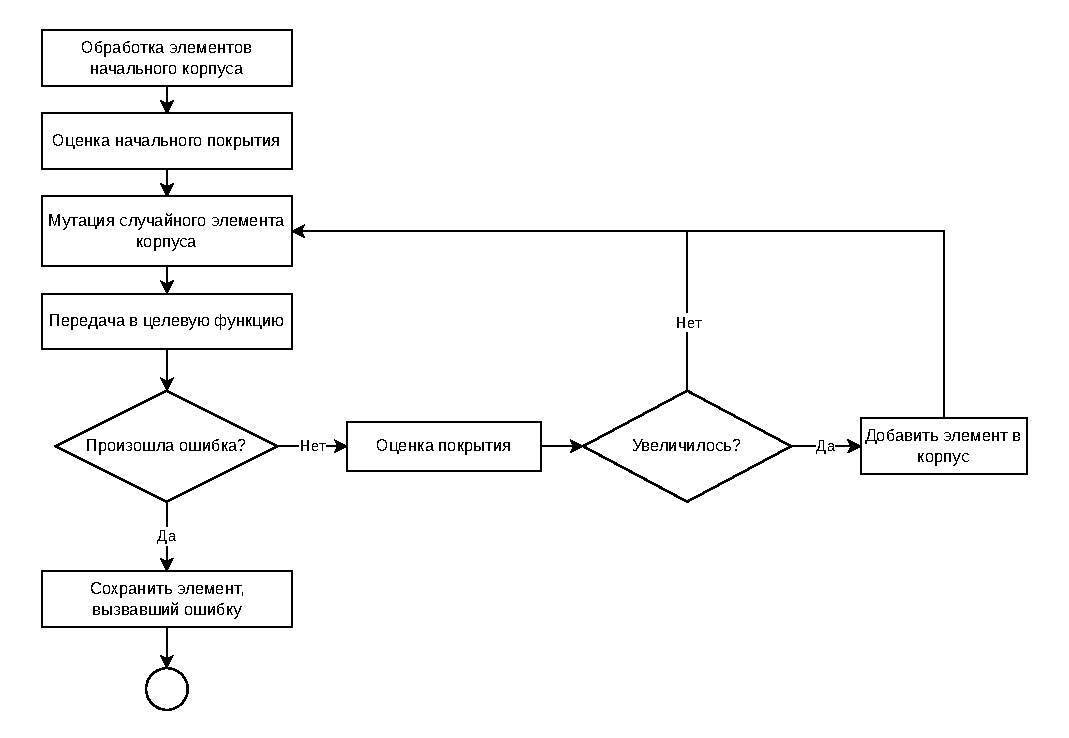
\includegraphics[width=0.8\textwidth]{Piclibfuzz.pdf} % Путь к файлу
	\caption{Общая схема работы фаззера с использованием libFuzzer.} % Подпись
	\label{pic:ilibfuzz} % Метка для ссылок
\end{figure}

Работа фаззера (см. рисунок \ref{pic:ilibfuzz}) начинается с инициализации корпуса, после чего запускается основной цикл: выбирается элемент из корпуса, мутирует, передается в целевую функцию и оценивается результат. В случае успешного увеличения покрытия или обнаружения ошибки (завершение с ошибкой, утечка памяти, таймаут) состояние сохраняется. Процесс продолжается бесконечно или прерывается в случае обнаружения ошибки. В последнем случае тест, вызвавший ошибку, сохраняется отдельно для последующего точечного воспроизведения.

Разработанный в рамках курсовой метод базируется на использовании серии сценариев работы с файловой системы. Так как драйвер NTFS является read-only, для ускорения фаззинга, был оставлен только один сценарий - сценарий рекурсивного обхода файловой системы, реализуемый двумя функциями:

\begin{itemize}
	\item \textbf{FsFuzzSubTest1} выполняет работу с отдельным файлом: открытие на чтение, чтение метаданных файла, последовательное чтение блоков данных с перемещением позиции, а затем открытие на запись для записи данных в конец файла. Алгоритм выявляет ошибки управления файловыми дескрипторами, обработки позиционирования и операций ввода-вывода. Обобщенная схема работы алгоритма представлена на рисунке \ref{pic:fsfuzzsubtesti}.
	\begin{figure}[htbp]
		\centering % Центрирование
		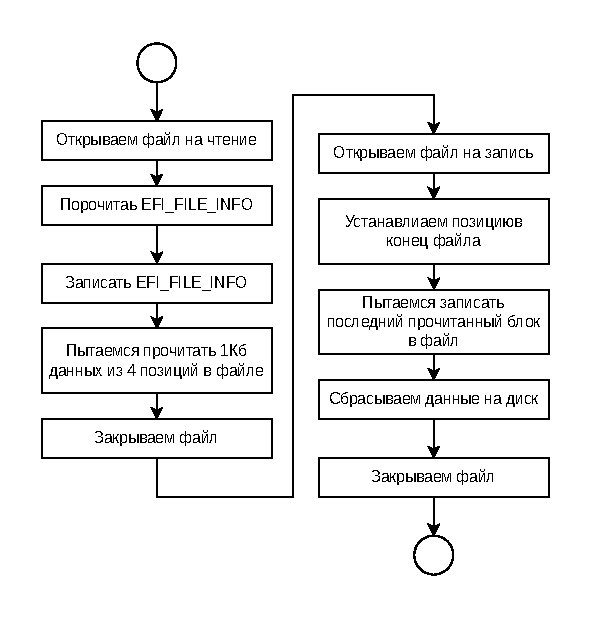
\includegraphics[width=0.5\textwidth]{FsFuzzSubtestI.pdf} % Путь к файлу
		\caption{Обобщенный алгоритм обработки файла \FunName{FsFuzzSubtest1}.} % Подпись
		\label{pic:fsfuzzsubtesti} % Метка для ссылок
	\end{figure}
\newpage
	\item \textbf{FsFuzzTest1} реализует рекурсивный обход файловой системы с заданной глубиной. Для каждого обнаруженного файла он запускает \FunName{FsFuzzSubtest1}, а для катологов - рекурсивно углубляется в иерархию. Обобщенная схема алгоритма представлена на рисунке \ref{pic:fsfuzztesti}.
	\begin{figure}[htbp]
		\centering % Центрирование
		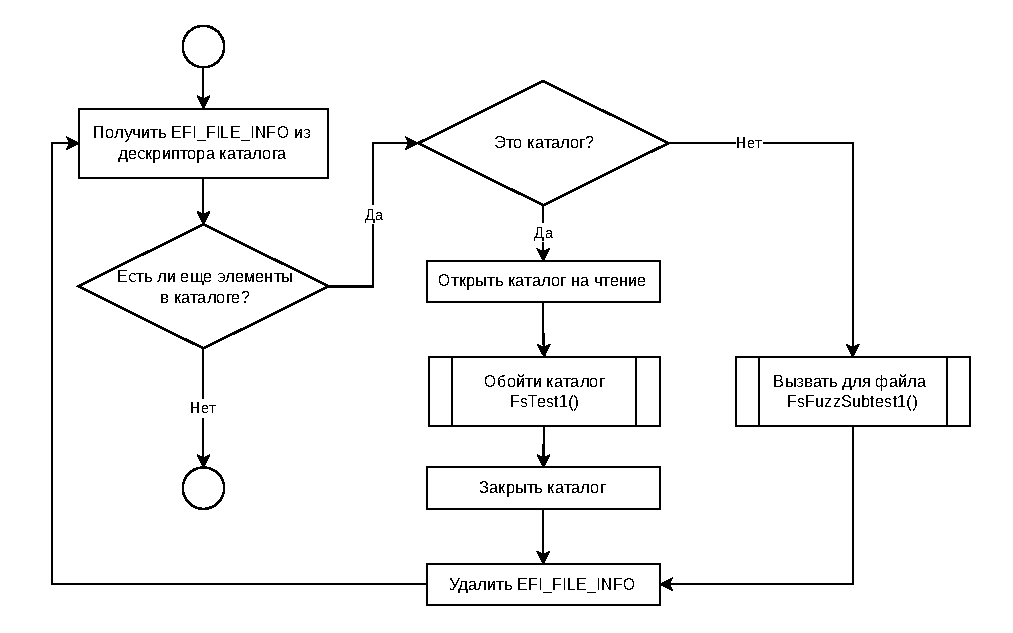
\includegraphics[width=0.7\textwidth]{FsFuzzTestI.pdf} % Путь к файлу
		\caption{Обобщенный алгоритм обхода каталога\FunName{FsFuzzTest1}.} % Подпись
		\label{pic:fsfuzztesti} % Метка для ссылок
	\end{figure}
\end{itemize}


\subsection{Создание начального корпуса}

В рамках курсовой работы была разработана серия bash-скриптов, создающая специализированные образы файловой системы NTFS. Подробные характеристики по каждому скрипту приведены в таблице \ref{tab:tests_detail}. Общие характеристики создаваемых образов:
\begin{itemize}
	\item Многоуровневые вложенные директории (до 4 уровней).
	\item Различные типы ссылок (символические и жесткие).
	\item Специальные случаи (ссылки на себя, корневые директории, за пределы образа).
	\item Различные размеры кластеров.
	\item Различные размеры образов (8 Мб - 32 Мб).
	\item Аналогичное заполнение до указанного порога (FILLSPACE, только Test1.sh).
	\item Генерация как стандартных, так и длинных имен со специальными символами.
	\item Жесткие ссылки на один файл.
\end{itemize} 

\begin{table}[htbp]
	\renewcommand{\arraystretch}{1.5}
	\centering
	\begin{tabular}{|c|c|p{10cm}|}
		\hline
		\textbf{Скрипт} & \textbf{Размер} & \textbf{Описание} \\
		\hline
		\textit{Test1.sh} & 16 Мб & Базовая структура: 4 корневые папки (по 10 файлов), 3 вложенные цепочки (глубина 3), 3 файла по 2 Мб в корне. FILLSPACE до 2 Мб. \\
		\hline
		\textit{Test2.sh} & 32 Мб & Нестандартный размер кластера (8 Кб). 5 корневых папок (по 15 файлов), 4 вложенные цепочки (глубина 4), 10 файлов по 1 Мб.\\
		\hline
		\textit{Test3.sh} & 32 Мб &Длинные имена (200 символов) со спецсимволами. 20 папок (по 200 файлов по 1 Кб) + символические ссылки на себя и из корня. \\
		\hline
		\textit{Test4.sh} & 8 Мб & Маленький образ. 20 папок (по 10 файлов по 1 Кб) + символические ссылки на себя в каждой папке и из корня на папки.\\
		\hline
		\textit{Test5.sh} & 16 Мб & Жесткие ссылки: 1 базовый файл (2 Мб) + 10 ссылок в корне + 5 ссылок в подпапке.\\
		\hline
		\textit{Test6.sh} & 16 Мб & Массовое создание файлов: 10 папок × 500 файлов (всего 5000). \\
		\hline
		\textit{Test7.sh} & 16 Мб & Папки с символическими ссылками: 5 папок (по 10 файлов), в каждой символические ссылки на себя и на корневую директорию.\\
		\hline
		\textit{Test8.sh} & 16 Мб & Символическая ссылка на внешнюю директорию: 5 папок (по 10 файлов), в каждой символические ссылки на себя, корень и внешнюю папку за пределами образа.\\
		\hline
	\end{tabular}
	\caption{Подробные характеристики скриптов для создания образов.}
	\label{tab:tests_detail}
\end{table}

Файловая система NTFS в своей архитектуре поддерживает сжатие файлов. Поэтому дополнительно были созданы 4 образа с атрибутами сжатия в среде ОС Microsoft Windows.  Серия образов, созданная скриптами и 4 дополнительных образа сжатой файловой системы образуют начальный корпус для фаззинг-тестирования.

\subsection{Результаты тестирования}

бла-бла-бла

\subsection{Покрытие кода}

бла-бла

\subsection{Подготовка и отправка патча с исправлениями}

бла-бла
